\section{Realizacja modułu Hough w sprzęcie}


%

\begin{figure}[!htb]
\centering
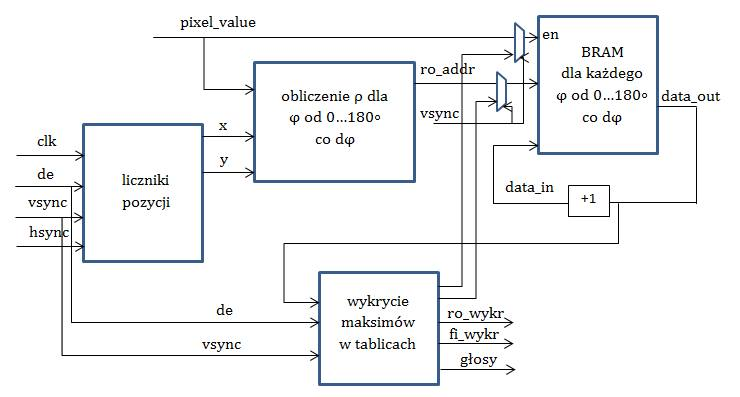
\includegraphics[scale=0.7]{img/schemat_hough.png}
\caption{Struktura modułu realizującego transformatę Hougha z wygaszaniem minimów na FPGA}
\label{rys:start1}
\end{figure}



